\documentclass[12pt,a4paper]{report}
\usepackage[utf8]{inputenc}
\usepackage[french]{babel}
\usepackage[T1]{fontenc}
\usepackage{amsmath}
\usepackage{amsfonts}
\usepackage{amssymb}
\usepackage{graphicx}
\usepackage{xcolor}
\usepackage{tikz}
\usepackage[pdfauthor={Alexandre MARIN}, pdfkeywords={IFPEN, Delaunay, Voronoi, mesh generation}, colorlinks=true, linkcolor=purple, urlcolor=blue, citecolor=magenta]{hyperref}
%\usepackage{pdfpages}

%\usepackage[nottoc,section]{tocbibind}
\usepackage{bibtopic}
\renewcommand{\thesection}{\arabic{section}}

\graphicspath{{pictures/}}

\begin{document}

\begin{titlepage}
\author{Alexandre \textsc{Marin}\\ Master Mathématiques et Applications Sorbonne Université\\ Parcours Ingénierie Mathématique\\ Majeure Ingénierie Mathématique Pour l'Entreprise}
\date{24/06 -- 30/10/2020\\ IFP \'Energies Nouvelles\\ Site de Rueil-Malmaison\\[1cm]Encadrants :\\Laurent \textsc{Astart}\\Alexandra \textsc{Bac}}
\title{Développement d’une bibliothèque de structures et algorithmes pour un mailleur polyédrique}
\maketitle
\end{titlepage}


\pagenumbering{gobble}
\section*{Remerciements}

Je remercie Laurent \textsc{Astart} de m'avoir accueilli à IFP \'Energies Nouvelles pour ce stage de fin d'études et je remercie Alexandra \textsc{Bac} de m'avoir co-encadré.

\tableofcontents
\newpage

\pagenumbering{arabic}

\section{Introduction}
%1 page
%ouverture
%annonce du plan
%position du stagiaire dans l'entreprise
Ce document est le rapport de mon stage qui a eu lieu à IFP \'Energies Nouvelles (IFPEN), et clôture donc ma seconde année de master à Sorbonne Université.

Ma position de stagiaire a été la suivante~: j'ai été intégré dans la direction scientifique \emph{Sciences et Technologies du Numérique}, et plus précisément dans le département \emph{Informatique Scientifique} du site de Rueil-Malmaison de IFPEN.

Ce rapport présente d'abord succinctement le déroulement du stage, expose ensuite son contexte en présentant l'entreprise, puis la mission du stage est détaillée et une quatrième partie apporte la conclusion.

Les informations qui concernent IFPEN ont été recueillies sur son site internet et sur l'intranet de l'entreprise.

\newpage
\section{Déroulement du stage}
%un paragraphe par mois
%une ou deux pages
Le premier mois du stage a été consacré à la découverte des locaux, à certaines formations obligatoires pour les nouveaux salariés (comme la formation sécurité) et à l'installation de logiciels nécessaires pour le stage. \`A la fin du mois de juillet, j'avais pris en main l'environnement de développement intégré QtCreator, j'avais développé en C++ une structure de données en demi-arêtes pour des maillages bidimensionnels et quelques classes outil pour générer des maillages de Delaunay.

Pendant le deuxième mois, le code C++ a été réorganisé dans le but d'ajouter plus facilement d'autres fonctionnalités comme le calcul de triangulations de Delaunay contraintes. De nombreux tests ont aussi été effectués pour vérifier la stabilité des programmes ainsi que la qualité des résultats.

Le rapport de stage a été composé lors du troisième mois. Entretemps, des diagrammes de Voronoï étaient générés et le code était amélioré.

Quant au dernier mois du stage, il a permis une seconde étude bibliographique portant, entre autres, sur des structures de données adaptées à des maillages polyédriques 3D.

\newpage
\section{Contexte et données générales}
%2-3 pages
Cette section a été composée à partir d'informations récupérées sur le site internet de IFPEN et sur son réseau intranet.
\vspace{1cm}

IFP \'Energies Nouvelles\footnote{L'ancienne dénomination était Institut Français du Pétrole jusqu'en 2010.} (IFPEN) est une entreprise du groupe du même nom : il s'agit d'un établissement public de recherche et de formation dans les domaines de l'énergie, du transport et de l'environnement, placé sous la tutelle du ministre chargé de l'énergie. Plus précisément, IFPEN est depuis 2006 un établissement public à caractère industriel et commercial (EPIC)\footnote{D'après l'article Wikipédia sur les EPICs, il s'agit \og d'une personne morale de droit public ayant pour but la gestion d'une activité de service public de nature industrielle et commerciale\fg{}.}. IFPEN est financé environ à moitié par l'\'Etat et crée lui-même plus de 50\% de son budget, notamment en valorisant le travail issu de la recherche. L'entreprise est présente sur deux sites : l'un à Rueil-Malmaison en \^Ile-de-France et l'autre à Solaize en Auvergne-Rhône-Alpes.

En 2019, IFPEN comptait $1\ 633$ salariés à temps plein, dont $1\ 136$ ingénieurs et techniciens R\&I (Recherche et Innovation), ainsi que près de $200$ allocataires de recherche, postdoctorants et stagiaires. Son budget atteignait $283,3$~\textrm{M}\texteuro. IFPEN déposait aussi $185$ brevets et était à l'origine de plus de $600$ publications scientifiques et communications à congrès.

IFPEN conçoit et développe des procédés, des équipements et des logiciels qui concernent quatre domaines : la mobilité durable, les énergies renouvelables, les hydrocarbures responsables, et le climat/l'environnement. Dans le domaine climat et environnement, l'une des problématiques est par exemple le captage, le stockage et l'utilisation du CO$_2$. Il s'agit de proposer aux industries lourdes (sidérurgie, cimenterie, raffinage, chimie, pétrochimie) des technologies pour réduire massivement leurs émissions de CO$_2$.

IFPEN collabore avec d'autres instituts de recherche et industries dans le cadre de partenariats qui sont de différents types. IFPEN est ses partenaires financent conjointement un projet de recherche et définissent les règles de propriétés des résultats grâce aux contrats de recherches bilatéraux ou aux consortiums dont certains sont des Joint Industry Project (JIP) : IFPEN y opère le programme R\&I et conserve la propriété industrielle. IFPEN participe aussi à des projets de recherche collaborative qui bénéficient de soutiens publics.

La plupart des entités de IFPEN, que l'on peut voir sur la figure \ref{ifpen_org}, se répartissent dans deux ensembles : \emph{les directions de recherche}, qui rassemblent les compétences scientifiques, et \emph{les directions fonctionnelles}, comme les ressources humaines, les finances ou le juridique.

Les programmes de recherche sont menés à travers des projets pouvant faire intervenir plusieurs directions de recherche et fonctionnelles. Ces mêmes projets sont pilotés par l'un des cinq centres de résultats qui s'occupent également de leur valorisation industrielle.

On trouve aussi dans l'entreprise une école d'ingénieurs, IFP School, ainsi que la direction générale. Il y a enfin un conseil d'administration, composé de seize membres dont quatre sont des représentants de l'\'Etat venant des ministères de l'énergie, de l'industrie, du budget et de la recherche.

\newpage
\section{Mission du stage}

\subsection{Objectifs}

Ce stage sert de prélude à la thèse \og \emph{Maillage polyédrique de volumes 3D optimisé pour la simulation en géosciences} \fg{}~: l'objectif de cette thèse est de proposer et confronter plusieurs stratégies de génération d'un maillage polyédrique du sous-sol à de nouveaux types de schémas numériques. Afin de rendre possibles des simulations concernant les problématiques du stockage du CO$_2$, la géothermie ou l'hydrogéologie, il faut représenter le plus fidèlement possible les discontinuités et hétérogénéités de la structure des sous-sols qui influencent beaucoup les transferts de masse et d'énergie. Il s'agit donc, étant donnée une description surfacique des éléments en jeu, de mailler un volume en respectant certaines contraintes, comme la conformité ou les rapports de forme des mailles.

Le premier objectif était, d'une part, d'effectuer un travail bibliographique sur la génération de maillages, et d'autre part, de créer une bibliothèque logicielle qui fournisse un maximum d'algorithmes et les structures de données nécessaires au développement du mailleur.

Cependant le véritable but du stage était l'appropriation de concepts liés à la génération de maillages 2D pour ensuite mieux saisir ceux relatifs à la génération de maillages 3D polyédriques.

\subsection{Travail effectué}

\subsubsection{\'Eléments théoriques pour les maillages}

On présente ici les triangulations de Delaunay, les triangulations de Delaunay contraintes pour mailler un domaine non nécessairement convexe, puis le dual des ces triangulations qui sont une piste pour l'obtention d'un maillage polyédrique ayant de bonnes propriétés.
\vspace{1cm}

Une \emph{triangulation de Delaunay} d'un ensemble de points $V\subset\mathbb{R}^2$ est un maillage conforme de l'enveloppe convexe de $V$, constitué de triangles satisfaisant la propriété du cercle vide~: le disque ouvert défini par le cercle circonscrit d'un triangle ne doit contenir aucun sommet de $V$. Ces triangles sont dits alors Delaunay. Parmi toutes les triangulations de $V$, celles qui sont Delaunay maximisent la valeur du plus petit angle formé par deux arêtes~: ce sont donc, pour cet ensemble $V$ et du point de vue de la qualité des mailles, les \og meilleures \fg{} triangulations. On peut voir un maillage Delaunay sur la figure \ref{delaunay}.

La propriété de ces maillages s'exprime aussi localement~: un maillage est Delaunay si et seulement si chaque arête est \emph{localement Delaunay}, \emph{i.e.} si chaque arête $e$ est au bord ou bien est la frontière commune de deux triangles $\tau_1$ et $\tau_2$ tels que le cercle circonscrit de $\tau_1$ n'englobe aucun sommet de $\tau_2$. Dans ce dernier cas, cela revient à dire qu'un cercle passant par les extrémités de $e$ n'englobe aucun sommet de $\tau_1$ et de $\tau_2$.
Une illustration de la propriété d'être localement Delaunay pour une arête se trouve sur la figure \ref{locDelaunay}. On y aperçoit les mêmes points et presque les mêmes arêtes à gauche et à droite, cependant l'arête $e$ ne relie pas les mêmes sommets. \`A gauche, un cercle passant par les deux extrémités de $e=\mathrm{AC}$ n'englobe ni $\mathrm{B}$ ni $\mathrm{D}$, donc $e$ est localement Delaunay (les arêtes et sommets n'appartenant pas aux triangles $\mathrm{ACD}$ et $\mathrm{ABC}$ ne doivent pas être pris en compte). Quant au dessin de droite, le cercle circonscrit du triangle $\mathrm{ABD}$ englobe $\mathrm{C}$, donc $e=\mathrm{BD}$ n'est pas localement Delaunay.

Lorsque l'on souhaite faire apparaître des arêtes spécifiques d'un ensemble $L$ dans le maillage à obtenir, on peut produire des maillages \emph{Delaunay contraints}~: il suffit pour cela de créer des maillages dont chaque arête est soit dans $L$, soit localement Delaunay. Les éléments de $L$ sont appelés des \emph{segments}. Plutôt que de mailler l'enveloppe convexe d'un nuage de point, on peut alors mailler un domaine qui n'est plus convexe et qui possède potentiellement des trous.
Pour définir ce qu'est un triangle Delaunay contraint, définissons d'abord la notion de \emph{visibilité} : \emph{grosso modo}, deux sommets $x$ et $y$ sont visibles l'un de l'autre si le segment ouvert $xy$ n'est pas intersecté par un segment $l\in L$ tel que $l\neq xy$.
Un triangle $\tau$ est alors dit \emph{Delaunay contraint} s'il satisfait la condition suivante : son cercle circonscrit n'englobe aucun sommet du maillage qui soit visible d'un point intérieur de $\tau$.
\vspace{1cm}

Le \emph{diagramme de Voronoï} d'un ensemble fini de points $V\subset\mathbb{R}^2$ est constitué d'un ensemble de cellules $V_p$ pour tout $p\in V$, définies par
\[V_p\ :=\ \left\{x\in\mathbb{R}^2\middle\vert\ \forall\,q\in V,\ \Vert x-p\Vert\leqslant\Vert x-q\Vert\right\}\text{.}\]
Il s'agit du dual de la triangulation de Delaunay $\mathcal{T}$ de $V$~: le diagramme de Voronoï relie les centres de cercle circonscrit des triangles de $\mathcal{T}$. Il existe toujours cependant des cellules de Voronoï qui sont infinies et délimitées aussi par des bissectrices des arêtes du bord de $\mathcal{T}$. De façon générale, les cellules $V_p$ sont des polygones convexes.

Lorsque l'on définit en plus l'ensemble des segments $L$ qui doivent apparaître dans le maillage $\mathcal{T}$, on s'intéresse plutôt au diagramme de Voronoï \emph{étendu} $\mathcal{V}$, défini dans \cite[pages 30-31]{Edelsbrunner}. Ici on ne représente que la \og feuille primale \fg{}~: on ne fait pas figurer des arêtes qui relient des centres de cercle circonscrit dans le diagramme $\mathcal{V}$ si elles intersectent un segment de $L$. Les sommets des cellules de Voronoï peuvent alors être des milieux de segments ou des intersections de bissectrices d'arêtes de $\mathcal{T}$ avec d'autres arêtes de $\mathcal{T}$.

Un exemple de diagramme de Voronoï obtenu avec la bibliothèque développée est visible sur la figure \ref{del_vor}.


\subsubsection{Structure de données en demi-arêtes}

Les maillages non structurés peuvent être représentés dans une structure compacte qui ne contient que les points ainsi que la liste des faces, elles-mêmes vues comme des listes de sommets. Mais une requête concernant des informations topologiques du maillage demande une préparation d'une autre structure de données représentant les adjacences, ce qui constitue un inconvénient majeur lorsque l'on veut des algorithmes efficaces~: par exemple, toute modification du maillage demande une mise à jour des informations d'adjacences.

Afin d'obtenir rapidement des données sur la \emph{topologie} du maillage, la structure de données en demi-arêtes a été mise en \oe{}uvre~: cela consiste à représenter le maillage par un graphe plan orienté. Chaque arête donne naissance à deux demi-arêtes, opposées l'une à l'autre, chacune pointant vers l'une des extrémités de l'arête. Pour se déplacer à l'intérieur de la structure de données, chaque demi-arête $he$ intérieure à une face $f$ pointe vers 
\begin{itemize}
\item une demi-arête qui part de la destination de $he$ et qui est intérieure à $f$ : on la nomme demi-arête suivante ;
\item la demi-arête qui lui est opposée, et qui est associée à la face $f'$ qui est adjacente à $f$ via l'arête matérialisée par $he$. Chaque demi-arête correspondant au bord est considérée comme intérieure à une face fictive de \og peau \fg{}.
\end{itemize}
Enfin chaque sommet $v$ pointe vers une demi-arête qui part de $v$.

Ainsi, il est aisé de se déplacer dans le maillage et l'on a accès instantanément à des informations topologiques. Par exemple, on peut facilement parcourir une partie de bord du maillage, connaître les voisins d'un sommet et les arêtes qui lui sont incidentes.

Les algorithmes de génération de maillage ont été écrits en tenant compte des avantages de cette structure.

La figure \ref{half_edge} illustre la structure en demi-arêtes.


\subsubsection{Structure de données accélératrice}

Les fonctions programmées étant censées générer de \og grands \fg{} maillages, des nuages de points très denses doivent être constitués~: la  complexité temporelle des algorithmes prend alors toute son importance. Par exemple, pour l'algorithme de Bowyer-Watson présenté en page \pageref{Bowyer-Watson}, la complexité dépend aussi d'une procédure de localisation de points dans une face du maillage ; dans le cas d'une recherche exhaustive, la complexité de l'étape de localisation est en $O(t)$, avec $t$ le nombre de triangles du maillage. On décide de remplacer cette procédure coûteuse en s'aidant d'un \emph{quadtree}, \emph{i.e.} un arbre quaternaire.

Le principe de la recherche est le suivant~: au préalable, on part d'une boîte $B$ censée englober le maillage et on convient du nombre maximal d'éléments pouvant être contenus dans une feuille de l'arbre. Chaque n\oe{}ud de l'arbre représente une région rectangulaire qui est une portion de la boîte englobante $B$. Lorsque qu'une feuille contient trop d'éléments, on lui crée quatre fils qui correspondent chacun à un quart de la zone représentée par l'ancienne feuille, puis on répartit les éléments dans les nouvelles feuilles selon leur position dans la région. Ainsi, la complexité de la recherche d'un élément selon sa position est en $O(h_{\text{quadtree}})$, avec $h_{\text{quadtree}}$ la hauteur de l'arbre construit.

Une illustration d'un quadtree se trouve en figure \ref{quadtree}.

\subsubsection{Algorithmique}

On peut citer quatre grandes familles d'algorithmes de génération de maillage :
\begin{description}
\item[les méthodes d'avancée de front] : les éléments sont intégrés un par un, en partant du bord du domaine afin de progresser vers son centre ;
\item[les procédures de raffinement] : elles insèrent soigneusement de nouveaux sommets afin de respecter des contraintes sur la qualité et la taille des éléments, tout en gardant une propriété du maillage de départ (comme celle d'être Delaunay)  ;
\item[les algorithmes de grilles] : à l'aide d'une grille, d'un quadtree ou d'un octree, une grille structurée est représentée pour servir de guide lors de la subdivision du domaine à mailler ;
\item[les algorithmes d'amélioration de maillage] : ils effectuent des opérations visant à optimiser localement un premier maillage.
\end{description}



Dans la bibliothèque à concevoir, on a ajouté des algorithmes qui construisent des maillages de Delaunay, contraints ou non. On y trouve les deux algorithmes principaux suivants.

\paragraph{\indent Algorithme de Bowyer-Watson}\label{Bowyer-Watson} : cette procédure incrémentale transforme un maillage Delaunay en une autre triangulation de Delaunay en insérant un nouveau sommet, par retriangulation locale. Les étapes sont :
\begin{enumerate}
\item localisation du nouveau sommet $s$ : trouver un triangle $\tau$ dont le cercle circonscrit contient $s$ ;
\item à partir de $\tau$, trouver de proche en proche tous les triangles qui ne satisfont plus la propriété du cercle vide à cause de $s$ ;
\item suppression des triangles trouvés ;
\item retriangulation de la cavité formée : chaque nouveau triangle doit avoir $s$ pour sommet et avoir une arête de la cavité pour côté.
\end{enumerate}
Avec une procédure de localisation efficace, on peut espérer une complexité en $O(n\log n)$, avec $n$ le nombre de sommets du maillage. Cet algorithme est plus rapide que celui présenté ci-après mais il nécessite d'avoir d'abord à disposition un maillage Delaunay. Par conséquent un domaine $D$ non convexe ne peut être maillé par cette procédure que si l'on est prêt à mailler un autre domaine $D'$ qui inclut $D$, dont il faut ensuite enlever les triangles qui n'appartiennent à $D$.

\paragraph{\indent Emballage cadeau (\emph{Gift-Wrapping})} : c'est un algorithme issu de la première classe citée qui maille un domaine défini par des polygones, des arêtes et des points, les éléments des deux derniers types devant apparaître dans le résultat. Le principe consiste à ajouter au fur et à mesure des triangles Delaunay contraints. Pour cela, on considère un ensemble $\mathcal{A}$ contenant des arêtes (orientées), initialisé au début avec les arêtes du bord du domaine. L'ensemble $\mathcal{A}$ est mis à jour à chaque insertion de triangle en fonction de ses côtés. L'algorithme prend fin lorsque $\mathcal{A}$ est vide, sinon une autre itération commence avec une arête $e\in\mathcal{A}$ et l'on cherche un sommet en entrée qui va former avec $e$ un triangle Delaunay contraint.

S'il y a $n$ sommets et $m$ segments à considérer en entrée, la complexité de cet algorithme est en $O(n^{2}m)$. Le principal avantage de cet algorithme est de pouvoir mailler directement un domaine qui n'est plus nécessairement convexe, cependant il peut être ralenti par de nombreux tests d'intersections et en pratique, le maillage résultant peut aussi contenir des trous.

\paragraph{Variantes} : on peut s'inspirer des algorithmes précédents pour insérer autrement un nouveau sommet dans une triangulation Delaunay (contrainte ou non) tout en conservant la propriété de Delaunay.

Pour insérer un sommet à l'extérieur d'un maillage Delaunay, il suffit d'ajouter certains triangles au bord du maillage à modifier et d'appeler la procédure Bowyer-Watson dans un ancien triangle du bord qui ne satisfait plus la propriété du cercle vide.

Pour ajouter un nouveau sommet dans une triangulation de Delaunay contrainte, il suffit d'invoquer l'algorithme de Bowyer-Watson, mais en permettant à la procédure de se déplacer de triangle en triangle adjacent uniquement lorsque l'arête frontière à traverser n'est pas un segment. De plus un cas particulier doit être traité : lorsque le nouveau sommet à insérer se situe sur un segment, il faut aussi diviser ce segment en deux autres segments et penser à appeler la procédure de Bowyer-Watson de part et d'autre de l'ancien segment.

Enfin, on peut ajouter un segment $l$ à une triangulation de Delaunay contrainte en supprimant toutes les arêtes dont l'intérieur intersecte $l$ puis en appliquant l'algorithme d'emballage cadeau aux deux cavités formées qui se touchent selon $l$. Une illustration de cette insertion de segment apparaît sur la figure \ref{inserting_a_segment}.

\vspace{1cm}
\subsubsection{Bibliographie et mise en \oe{}uvre informatique}

La bibliographie servant de point de départ se trouve à la fin du rapport, en page \pageref{biblio}. L'article \cite{Garimella} décrit une procédure qui génère des maillages de volumes séparés par des interfaces, à partir des diagrammes de Voronoï. Puisqu'il faut au préalable déterminer des triangulations de Delaunay, les notes \cite{delnotes} ont été lues pour avoir à disposition des algorithmes de génération de maillages de Delaunay. Le livre \cite{Edelsbrunner} complète les deux premières références, en donnant par exemple la définition des diagrammes de Voronoï étendus pour les maillages de Delaunay contraints.

\vspace{1cm}

La bibliothèque logicielle à créer a été programmée en C++ à l'aide de l'environnement de développement intégré QtCreator \cite{QtCreator}, sous Windows. La compilation y est automatisée grâce à des fichiers de type \verb+Makefile+, générés après l'analyse par le programme \verb+QMake+ de fichiers projets \verb+.pro+ (un par sous-projet et un pour le projet global).
Cette bibliothèque est découpée en plusieurs sous-projets que l'on présente ici~:
\begin{description}
\item[noyau géométrique (GeometricCore)]~: cela permet d'effectuer des calculs en géométrie. La bibliothèque Eigen \cite{Eigen} écrite en C++ a été incorporée au projet pour faire de l'algèbre linéaire ;
\item[maillages bidimensionnels (MeshCore)]~: on utilise la structure en demi-arêtes pour représenter les maillages dans le plan. D'autres classes modélisant des concepts ayant trait aux maillages y figurent, comme des propriétés concernant des faces ou des arêtes ;
\item[entrées/sorties (MeshIO)]~: afin de visualiser ou réutiliser des maillages, l'importation et/ou l'exportation a été codée pour les formats \verb+OBJ+, \verb+PLY+ et \verb+XDMF+\footnotemark \footnotetext{\texttt{XDMF} (eXtensible Data Model and Format) est un dialecte de \texttt{XML} permettant de renseigner des polyèdres généraux. Le format est décrit à l'adresse \url{http://www.xdmf.org/index.php/XDMF\_Model\_and\_Format} .} ;
\item[Delaunay]~: ce projet fournit des algorithmes pour générer des triangulations de Delaunay et de Delaunay contraintes ;
\item[Voronoï]~: ce projet permet de calculer des diagrammes de Voronoï ;
\item[Test]~: dans ce dernier sous-projet, on y prépare des cas tests pour valider les programmes et pour s'assurer que ces derniers sont stables, rapides et/ou suffisamment précis.
\end{description}



Un certain nombre de mécanismes du C++ ont été utilisés pour ajouter de la clarté au projet. Chaque module de la bibliothèque contient plusieurs fichiers sources et en-têtes où sont définies des classes, les interactions entre ces dernières étant régies par l'ajout de méthodes, le réglage des visibilités des membres de classes, ou encore par une technique de création de clé, nécessaire pour invoquer une méthode, mais que seules certaines classes peuvent se procurer. Dans la mesure du possible, les concepts étaient modélisés par des classes ; les méthodes qui prenaient en argument une fonction étaient codées comme des patrons que l'on utilisait par exemple grâce à des \emph{lambda}.

La classe maillage manipule des indices pour référencer les sommets, demi-arêtes et faces, or la structure de données évolue beaucoup à cause d'ajouts et suppressions répétés d'éléments. Il a fallu donc avoir à disposition une classe \og vecteur à trous \fg{} qui gère elle-même la modification du contenu d'une zone mémoire contiguë : les cases vides sont réutilisées dès que possible et les indices permettant de retrouver les éléments des vecteurs restent inchangés pendant tout le programme.

Les tests se sont avérés essentiels : un fichier de test par sous-projet a été écrit. On y appelle les méthodes publiques des classes principales pour construire par exemple des maillages simples, mais de temps en temps dans la mesure du possible on essaye de considérer plusieurs cas limites. On prépare aussi des \emph{tests unitaires} pour vérifier le bon fonctionnement d'algorithmes et structures de données, indépendamment des autres éléments du programme. Par exemple, différentes configurations ont été considérées pour vérifier si le programme parvenait à savoir quand deux segments ouverts s'intersectaient.

\vspace{1cm}
La gestion de version s'est faite grâce à l'outil Git \cite{Git}.
L'architecture du projet est visible sur la figure \ref{archi} et quelques données sur le projet sont regroupées dans la figure \ref{stats}.

\subsubsection{Seconde étude bibliographique}

D'autres références à propos des maillages ont été lues : certaines décrivent une structure de données pour représenter un maillage polyédrique, d'autres proposent des méthodes de génération de maillages 3D destinés à des simulations en géosciences. Cette seconde bibliographie est donnée en page \pageref{second_biblio}.

\subsection{Résultats}

Des images sont fournies en annexe pour illustrer quelques résultats issus de l'exécution des tests. On montre des triangulations de Delaunay, Delaunay contraintes ainsi que des diagrammes de Voronoï sur les figures \ref{del_vor} et \ref{sq_del_vor}. Une triangulation de Delaunay contenant $100\ 000$ points tirés aléatoirement peut être engendrée en moins de $10$ secondes. La plupart du temps, lorsqu'un grand nombre de points devaient être insérés dans un maillage, la position des points était tirée aléatoirement de façon uniforme, mais aussi de manière à éviter que des points ne se situent au bord du domaine et conduisent à la création de triangles dégénérés.

Certaines figures ont été créées grâce au format \verb+PLY+ : sur la figure \ref{cut_segments} on constate la préservation des segments dans un maillage Delaunay contraint. Quant aux figures \ref{simple_Delaunay}, \ref{two_segments} et \ref{five_segments}, elles mettent en évidence la capacité du programme à ajouter des segments dans un maillage Delaunay, contraint ou non.

\subsection{Problèmes rencontrés}

%visualisation-couleurs
%bogues
La principale difficulté a été la vérification des fonctions programmées par la visualisation des résultats obtenus. Différents logiciels ont été utilisés, comme Paraview, CloudCompare ou MeshLab \cite{Paraview, CloudCompare, MeshLab}, mais ils n'interprètent pas tous les mêmes formats de fichier et ils peuvent rendre compte des maillages très différemment. Par exemple, le format \verb+PLY+ permet de renseigner des couleurs attachées à des points, arêtes et faces ; cependant ces données ne sont pas toujours acceptées et souvent les éléments sont coloriés par interpolation des couleurs des extrémités, ce qui ne correspond pas tout le temps à ce que l'on veut obtenir. Néanmoins ces couleurs se sont révélées pratiques quand il a fallu afficher des propriétés comme celle d'être localement Delaunay pour une arête.

De surcroît, certaines fonctions ne peuvent pas être visualisées simplement. Pour la structure en demi-arêtes, un bogue a été découvert pendant le deuxième mois du stage. En effet, un cas particulier n'avait pas été traité lorsque deux faces doivent être collées, et la connectivité était perdue parce qu'on ne pouvait parfois plus déduire toutes les arêtes incidentes à un sommet à partir de ce dernier.

Une dernière difficulté était l'adaptation d'algorithmes qui étaient exacts en théorie mais qui ne fonctionnaient pas bien en pratique à cause de l'arithmétique des nombres à virgule flottante. Quand un sommet à ajouter avec l'algorithme de Bowyer-Watson se situait très près d'un segment, il fallait prendre une décision : soit ajouter un triangle presque dégénéré, soit diviser le segment en deux autres segments. Or il n'est pas simple de savoir si le nouveau sommet appartient au segment ou pas, et comme des triangles très plats peuvent quand même apparaître dans une triangulation de Delaunay, il n'est pas non plus évident de savoir quand un triangle doit être jugé \og trop plat\fg{}.

\newpage
\section{Conclusion}

Le travail effectué pendant ce stage m'a permis, d'une part, de me perfectionner en programmation en réfléchissant pendant plusieurs mois à l'élaboration d'une bibliothèque, et d'autre part, de découvrir des méthodes pour générer et représenter des maillages 2D et 3D.

La dépendance des formes des cellules de Voronoï vis-à-vis des sommets des triangulations de Delaunay n'a pas été étudiée. Or le placement des sommets pour lesquels on génère le diagramme de Voronoï est crucial pour obtenir de bons rapports de forme des mailles. Bien positionner les sommets de départ permet en outre de s'éloigner des conditions qui amènent par exemple au problème d'ajout de sommet près d'un segment, décrit à la sous-section précédente. Il sera peut-être nécessaire de s'intéresser à des méthodes d'optimisation de maillages si la qualité des premiers maillages volumiques n'est pas satisfaisante.

Grâce aux difficultés rencontrées, théoriques et pratiques, je peux à présent mieux mesurer la complexité de la mission dans laquelle s'inscrit la thèse correspondante. Cette dernière sera l'occasion de trouver de bonnes propriétés pour des maillages 3D polyédriques, afin de résoudre des équations aux dérivées partielles modélisant des écoulements en milieu poreux.

Enfin, ce stage constitue une expérience professionnelle supplémentaire qui m'a fait connaître une entreprise dont les missions liées aux domaines de l'énergie et de l'environnement sont d'actualité et font partie d'un secteur d'avenir.

\newpage
\section{Annexes}

\begin{figure}[htbp]
\begin{center}
\usetikzlibrary {shapes.geometric}
\begin{tikzpicture}[fill=blue!20]
%\draw[help lines] (-1,-2) grid (6,3);
\path (0,0)
(10,0) node(c) [rectangle,draw,fill] {GeometricCore}
(5,0) node(d) [rectangle,draw,fill] {MeshCore}
(2,2) node(e) [rectangle,draw,fill] {MeshIO}
(2,0) node(f) [rectangle,draw,fill] {Delaunay}
(2,-2) node(g) [rectangle,draw,fill] {Voronoi}
(2,-4) node(h) [rectangle,draw,fill] {Test};
\draw[thick, ->] (d) |- (c);
\draw[thick,->] (h) -| +(-2,0) |- (f) ;
\draw[thick,->] (h) -| +(-2,0) |- (e) ;
\draw[thick,->] (h.north) -- (g) ;
\draw[thick,->] (h.east) -- (d) ;
\draw[thick,->] (h.east) -- (c) ;
\draw[thick,->] (e) -- (d) ;
\draw[thick,->] (f) -- (d) ;
\draw[thick,->] (g) -- (d) ;
\draw[thick,blue,->] (f) .. controls +(down:1.5cm) .. (c);
\draw[thick,blue,->] (g.east) .. controls +(right:1.5cm) .. (c);
\end{tikzpicture}
\caption{Architecture du projet~: les flèches indiquent les dépendances d'un sous-projet à un autre, qu'il faut considérer lors de la compilation. Le sous-projet \texttt{Test} permet de construire un exécutable tandis que les autres sous-projets correspondent à des bibliothèques.}
\label{archi}
\end{center}
\end{figure}

\begin{figure}
\begin{center}
\begin{tabular}{|l|c|}\hline
Fichiers C++ écrits & $29$ \\\hline
Lignes & $\approx 5000$\\\hline
Classes & $41$\\\hline
Nombre moyen de méthodes par classe & $7,8$\\\hline
\end{tabular}
\caption{Quelques statistiques sur le code produit.}
\label{stats}
\end{center}
\end{figure}
\clearpage

\begin{figure}[htbp]
\begin{center}
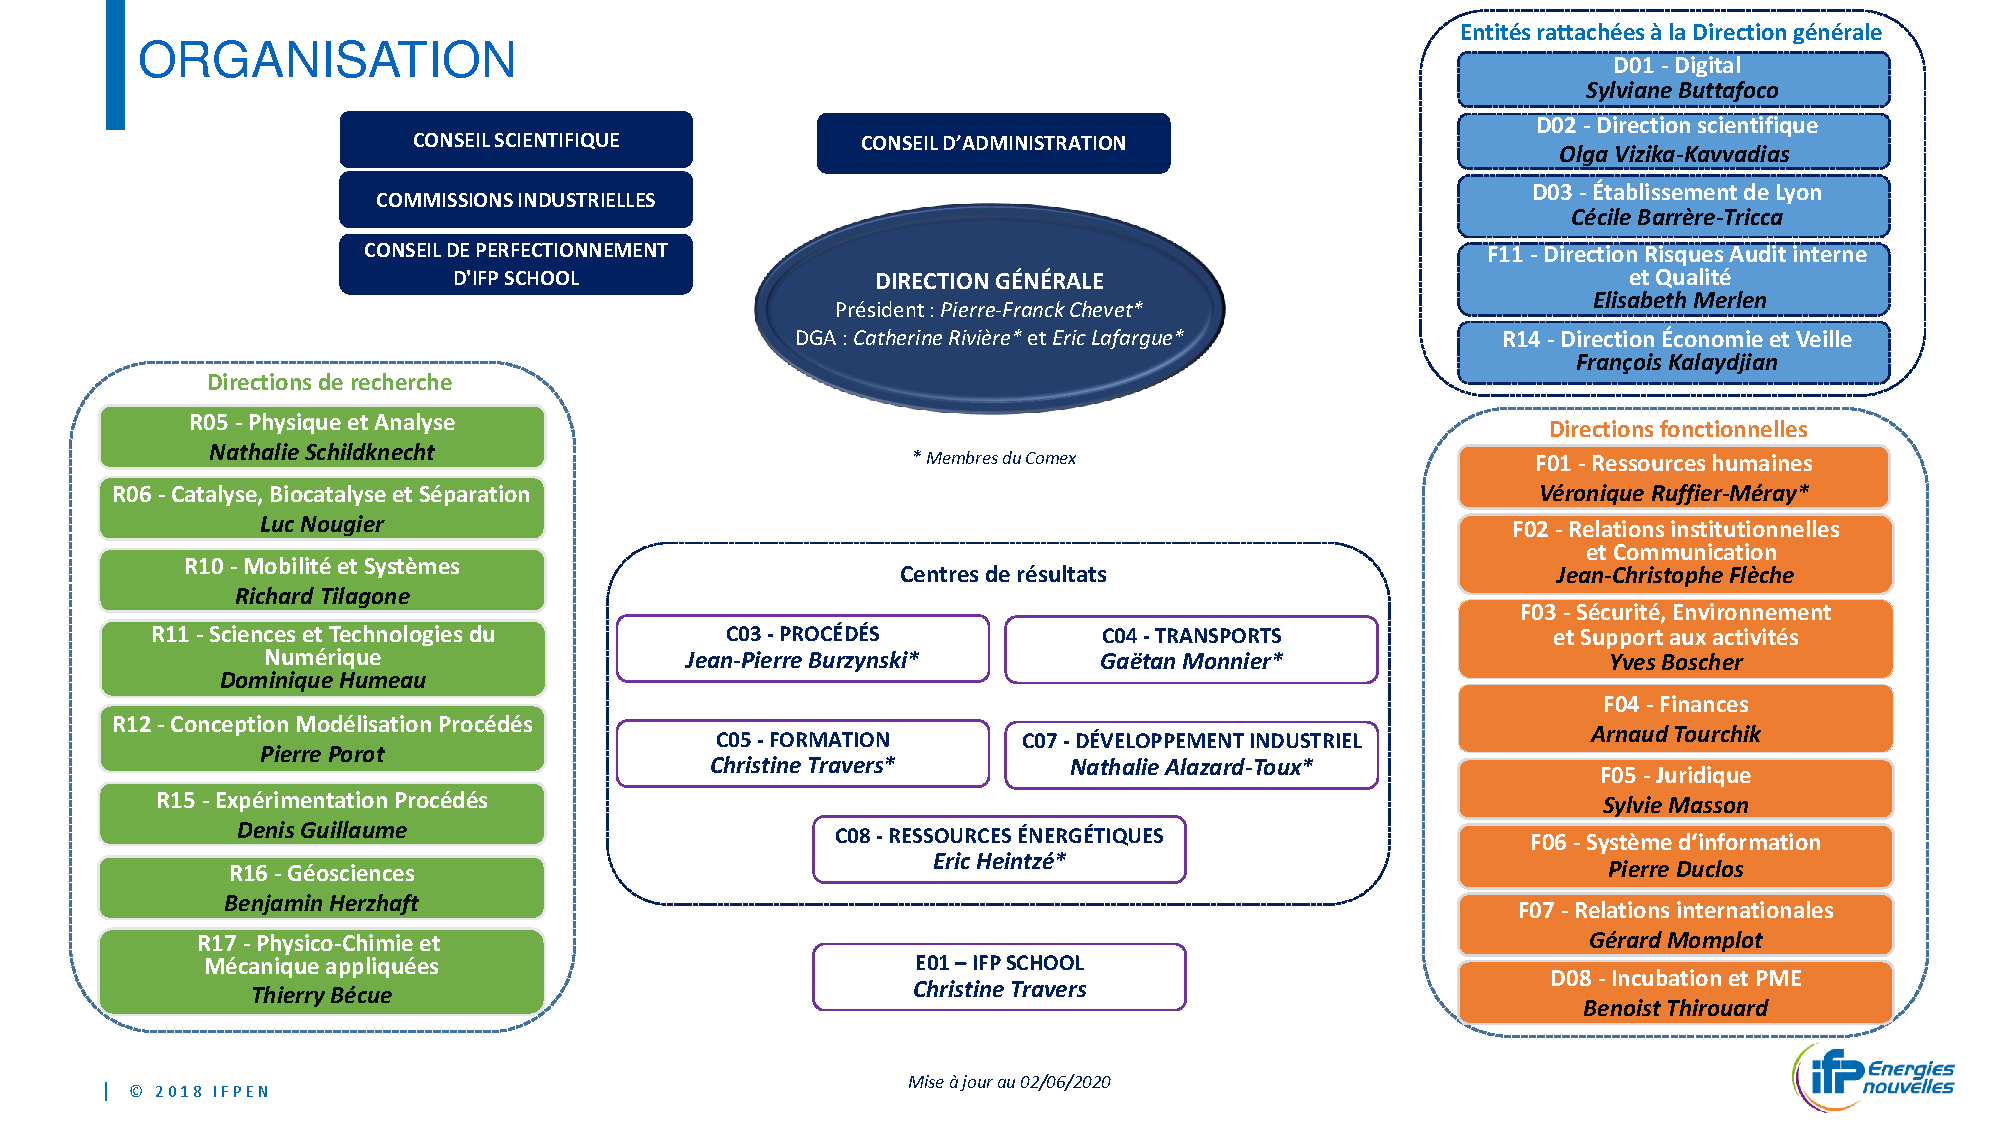
\includegraphics[scale=0.6, angle=90]{vf-schema-organisation-ifpen-marguerite.pdf}
\caption{Schéma de l'organisation de IFPEN (source : intranet de IFPEN).}
\label{ifpen_org}
\end{center}
\end{figure}
\clearpage

\begin{figure}[t]
\begin{center}
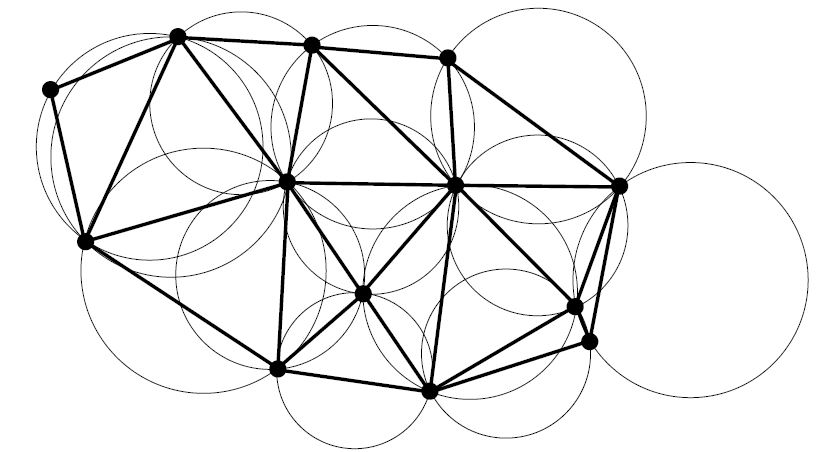
\includegraphics[scale=0.6]{delTri.jpg}
\caption{Figure 2.3 de la source \cite{delnotes} : exemple de triangulation de Delaunay. Les cercles circonscrits des triangles sont dessinés et permettent de voir que chaque triangle possède bien la propriété du cercle vide.}
\label{delaunay}
\end{center}
\end{figure}

\begin{figure}[h]
\begin{center}
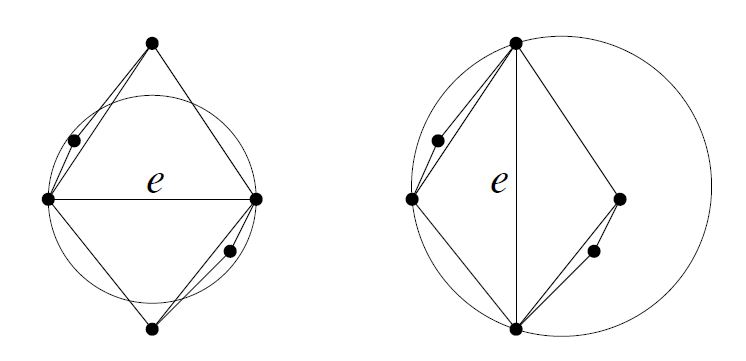
\includegraphics[scale=0.65]{locDel.jpg}
\caption{Figure 2.7 de la source \cite{delnotes} : l'arête $e$ est localement Delaunay à gauche mais ne l'est pas à droite.}\label{locDelaunay}\vspace{-3.5cm}\hspace{-10cm}A

\vspace*{1.2cm}\hspace{-6cm}B

\vspace*{-5.2cm}\hspace{-6cm}D

\vspace*{2cm}\hspace{-2.7cm}C
\end{center}
\end{figure}


\begin{figure}[htbp]
\begin{center}
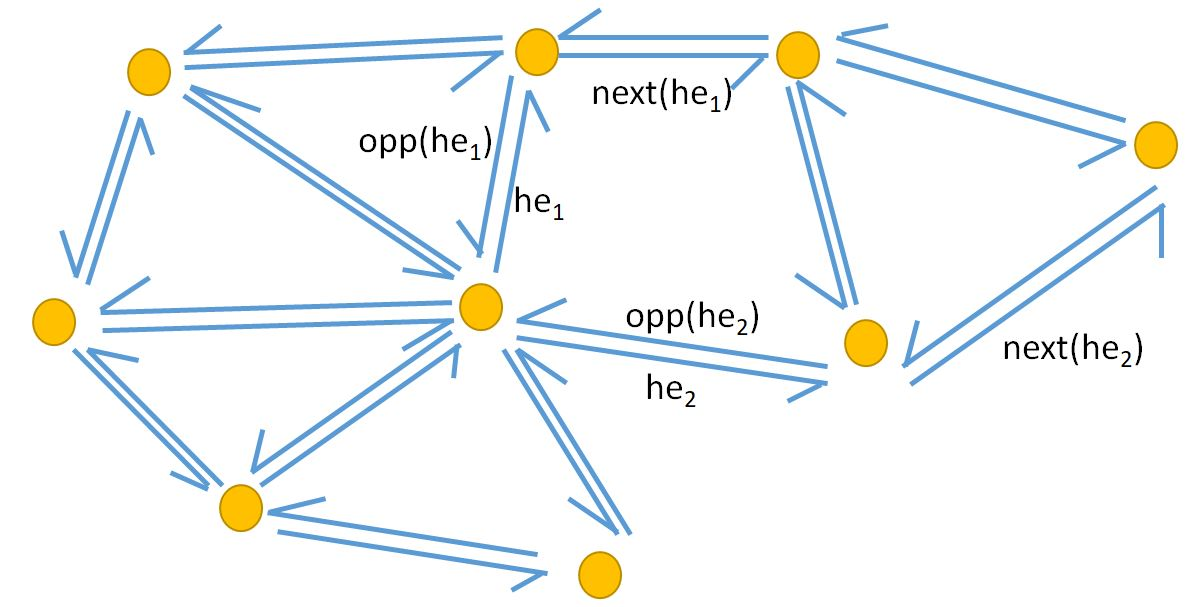
\includegraphics[scale=0.5]{halfEdge.jpg}
\caption{Représentation avec demi-arêtes d'un maillage contenant six polygones : les demi-arêtes correspondent aux flèches bleues. Ici on a indiqué la demi-arête suivante (\emph{next}) et opposée (\emph{opp}) pour deux demi-arêtes $\mathrm{he}_1$ et $\mathrm{he}_2$.}
\label{half_edge}
\end{center}
\end{figure}


\begin{figure}[htbp]
\begin{center}
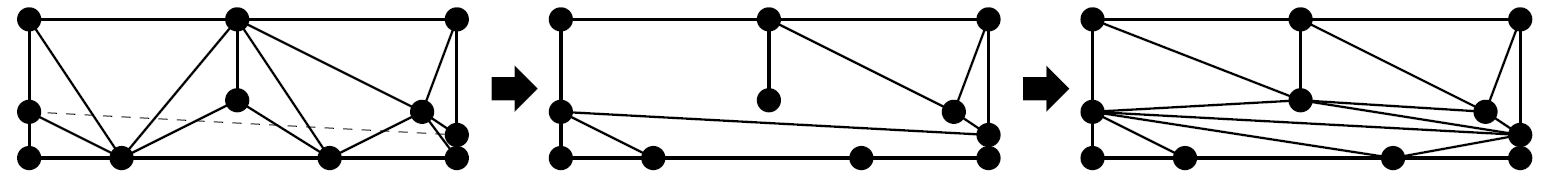
\includegraphics[scale=0.4]{insertingASegment.jpg}
\caption{Figure 2.16 de la source \cite{delnotes} : de gauche à droite, on identifie les arêtes intersectées par le nouveau segment $l$ en pointillés, on supprime ensuite ces arêtes puis on triangule les deux cavités qui se trouvent de part et d'autre de $l$. Parfois, comme dans le dessin du milieu, il reste des arêtes isolées qui sont en fait des segments, qui doivent bien sûr apparaître dans le résultat final.}
\label{inserting_a_segment}
\end{center}
\end{figure}
%\clearpage

\begin{figure}[t]
\begin{center}
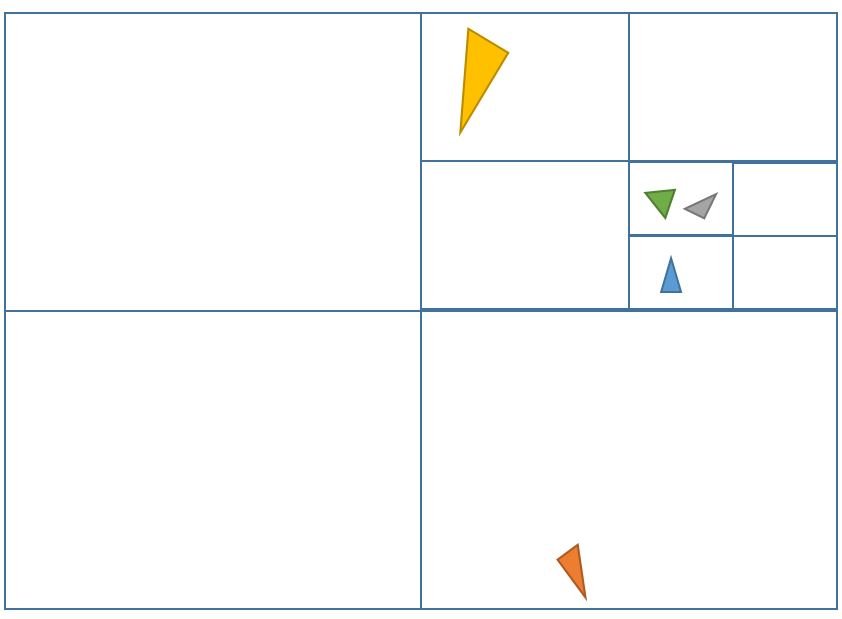
\includegraphics[scale=0.5]{boundingBoxes.jpg}
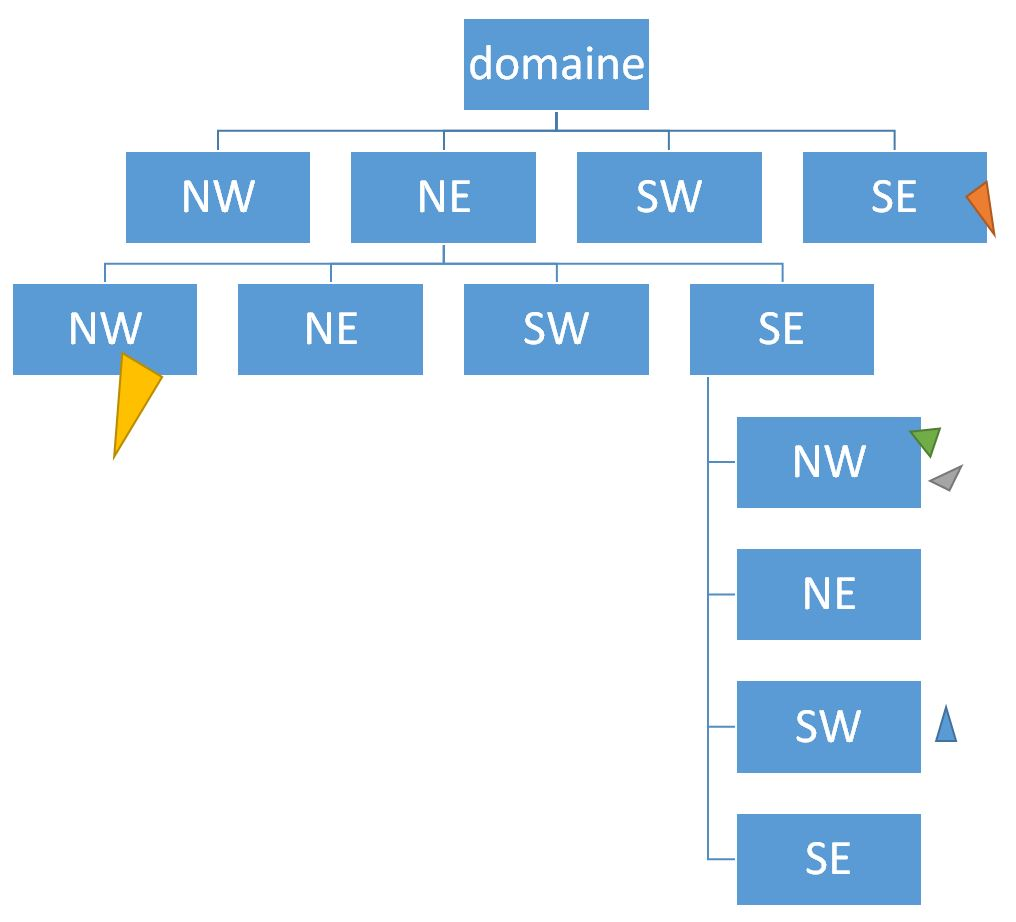
\includegraphics[scale=0.45]{quadtree.jpg}
\caption{Exemple de quadtree : en haut, des faces avec des boîtes englobantes sont illustrées, et un schéma de l'arbre correspondant se trouve en bas. La racine est associée à la plus grande boîte rectangulaire tandis que les autres n\oe{}uds symbolisent des sous-régions. Deux points cardinaux sont utilisés pour identifier le quart de la boîte associée au n\oe{}ud parent. Chaque triangle est mis à proximité de la feuille dans laquelle il est contenu.}\label{quadtree}
\end{center}
\end{figure}


\begin{figure}[t]
\begin{center}
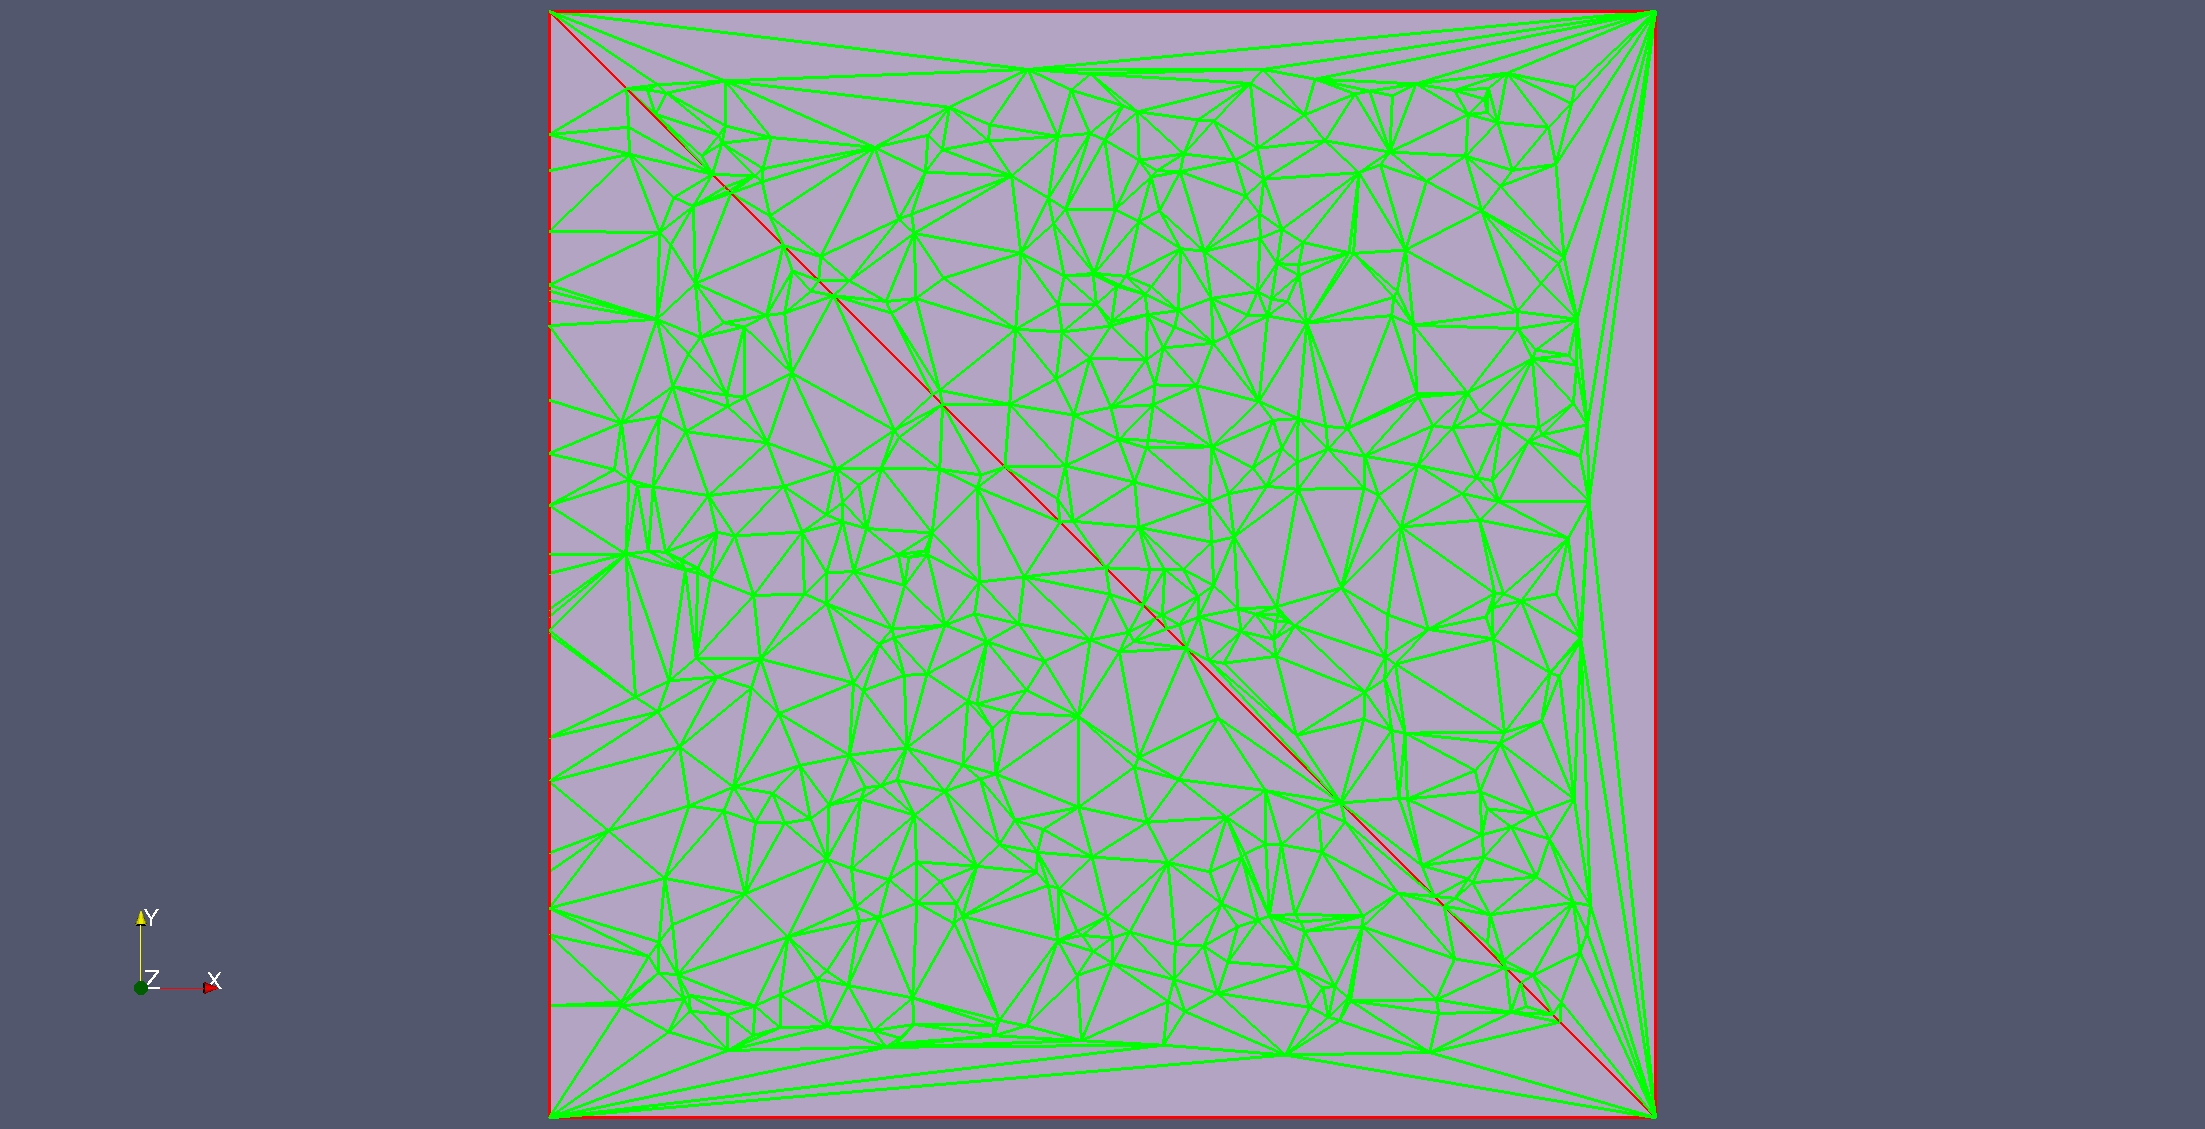
\includegraphics[scale=0.35, viewport=530 0 1680 1129, clip]{cutSegments.jpg}
\caption{Maillage Delaunay contraint dont les segments d'origine ont été divisés par ajout de sommets. On distingue encore la diagonale et le côté gauche du carré est resté bien rectiligne. Les arêtes coloriées en vert sont localement Delaunay.}\label{cut_segments}
\end{center}
\end{figure}

\begin{figure}[t]
\begin{center}
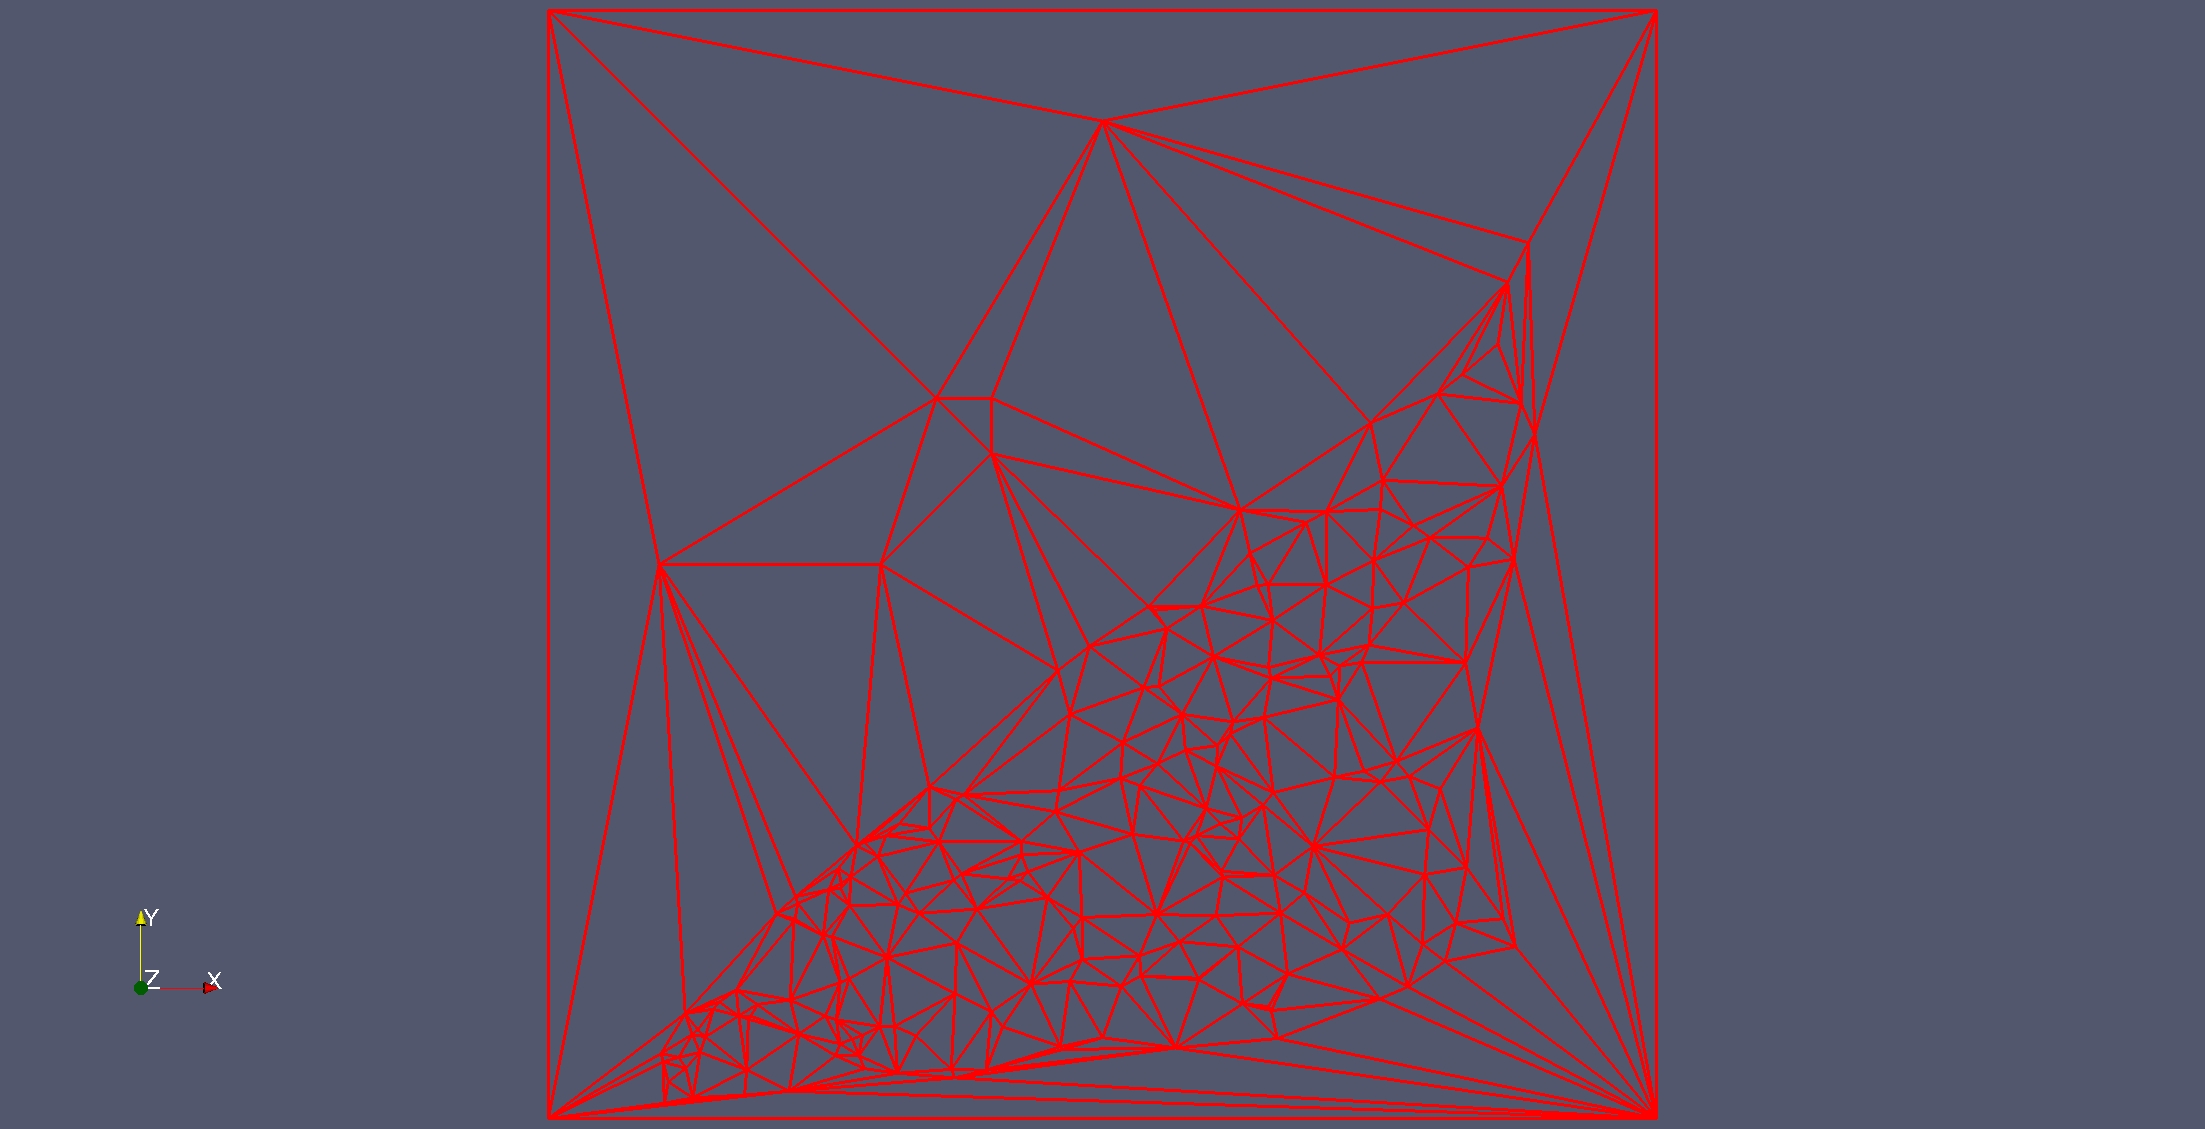
\includegraphics[scale=0.35, viewport=500 0 1680 1129, clip]{simpleDelaunay.jpg}
\caption{Maillage Delaunay d'un carré, auquel des segments vont être ajoutés.}\label{simple_Delaunay}
\end{center}
\end{figure}

\begin{figure}[t]
\begin{center}
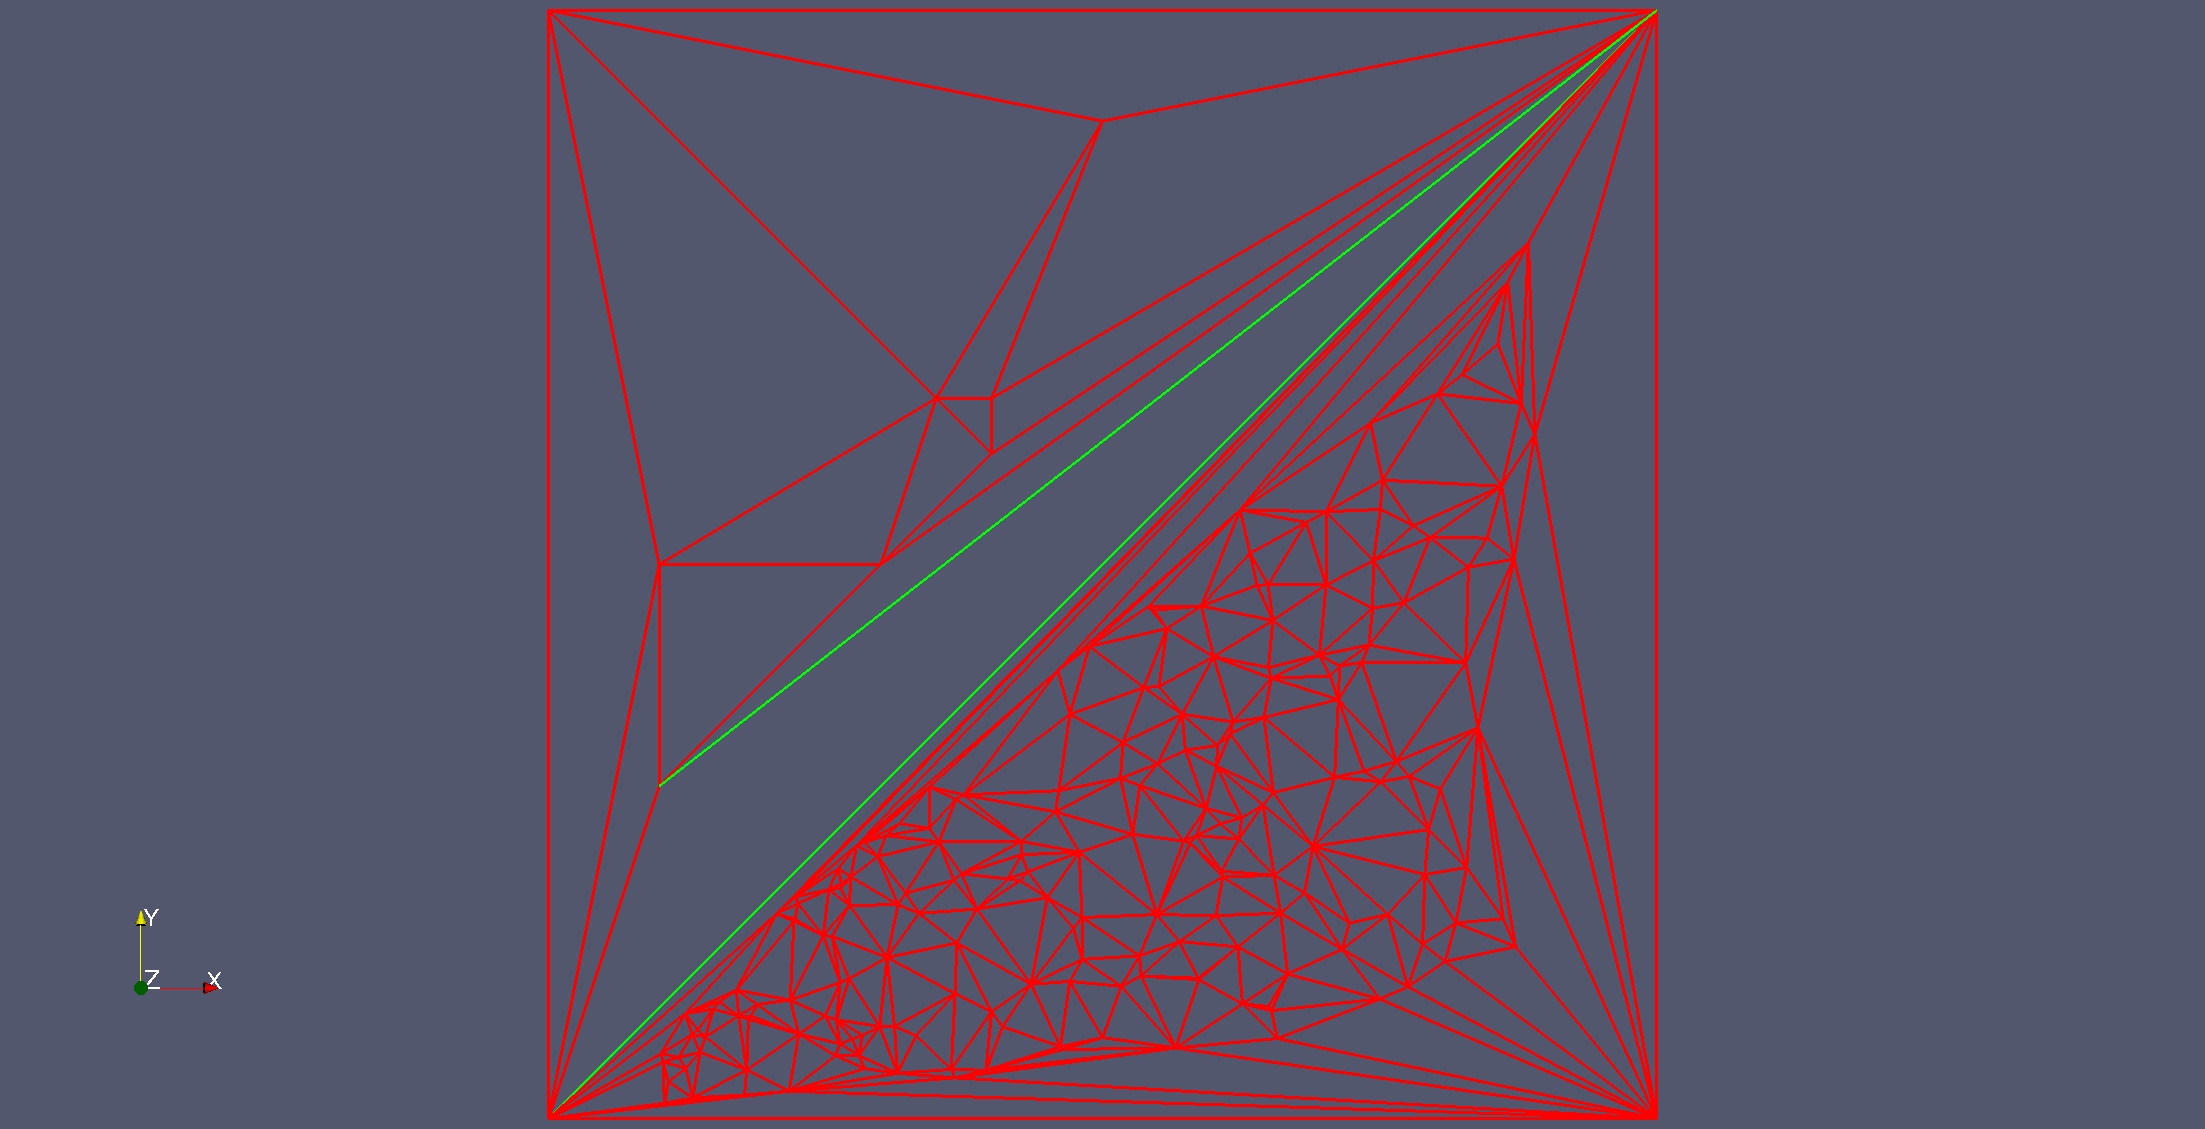
\includegraphics[scale=0.35, viewport=500 0 1680 1129, clip]{two_segments.jpg}
\caption{Maillage Delaunay contraint contenant deux segments (coloriés en vert, sous Paraview), obtenu par modification de la triangulation de la figure \ref{simple_Delaunay}. On constate que les changements effectués sont locaux puisque les triangles de la précédente triangulation qui sont loin des segments ont été conservés.}\label{two_segments}
\end{center}
\end{figure}

\begin{figure}[t]
\begin{center}
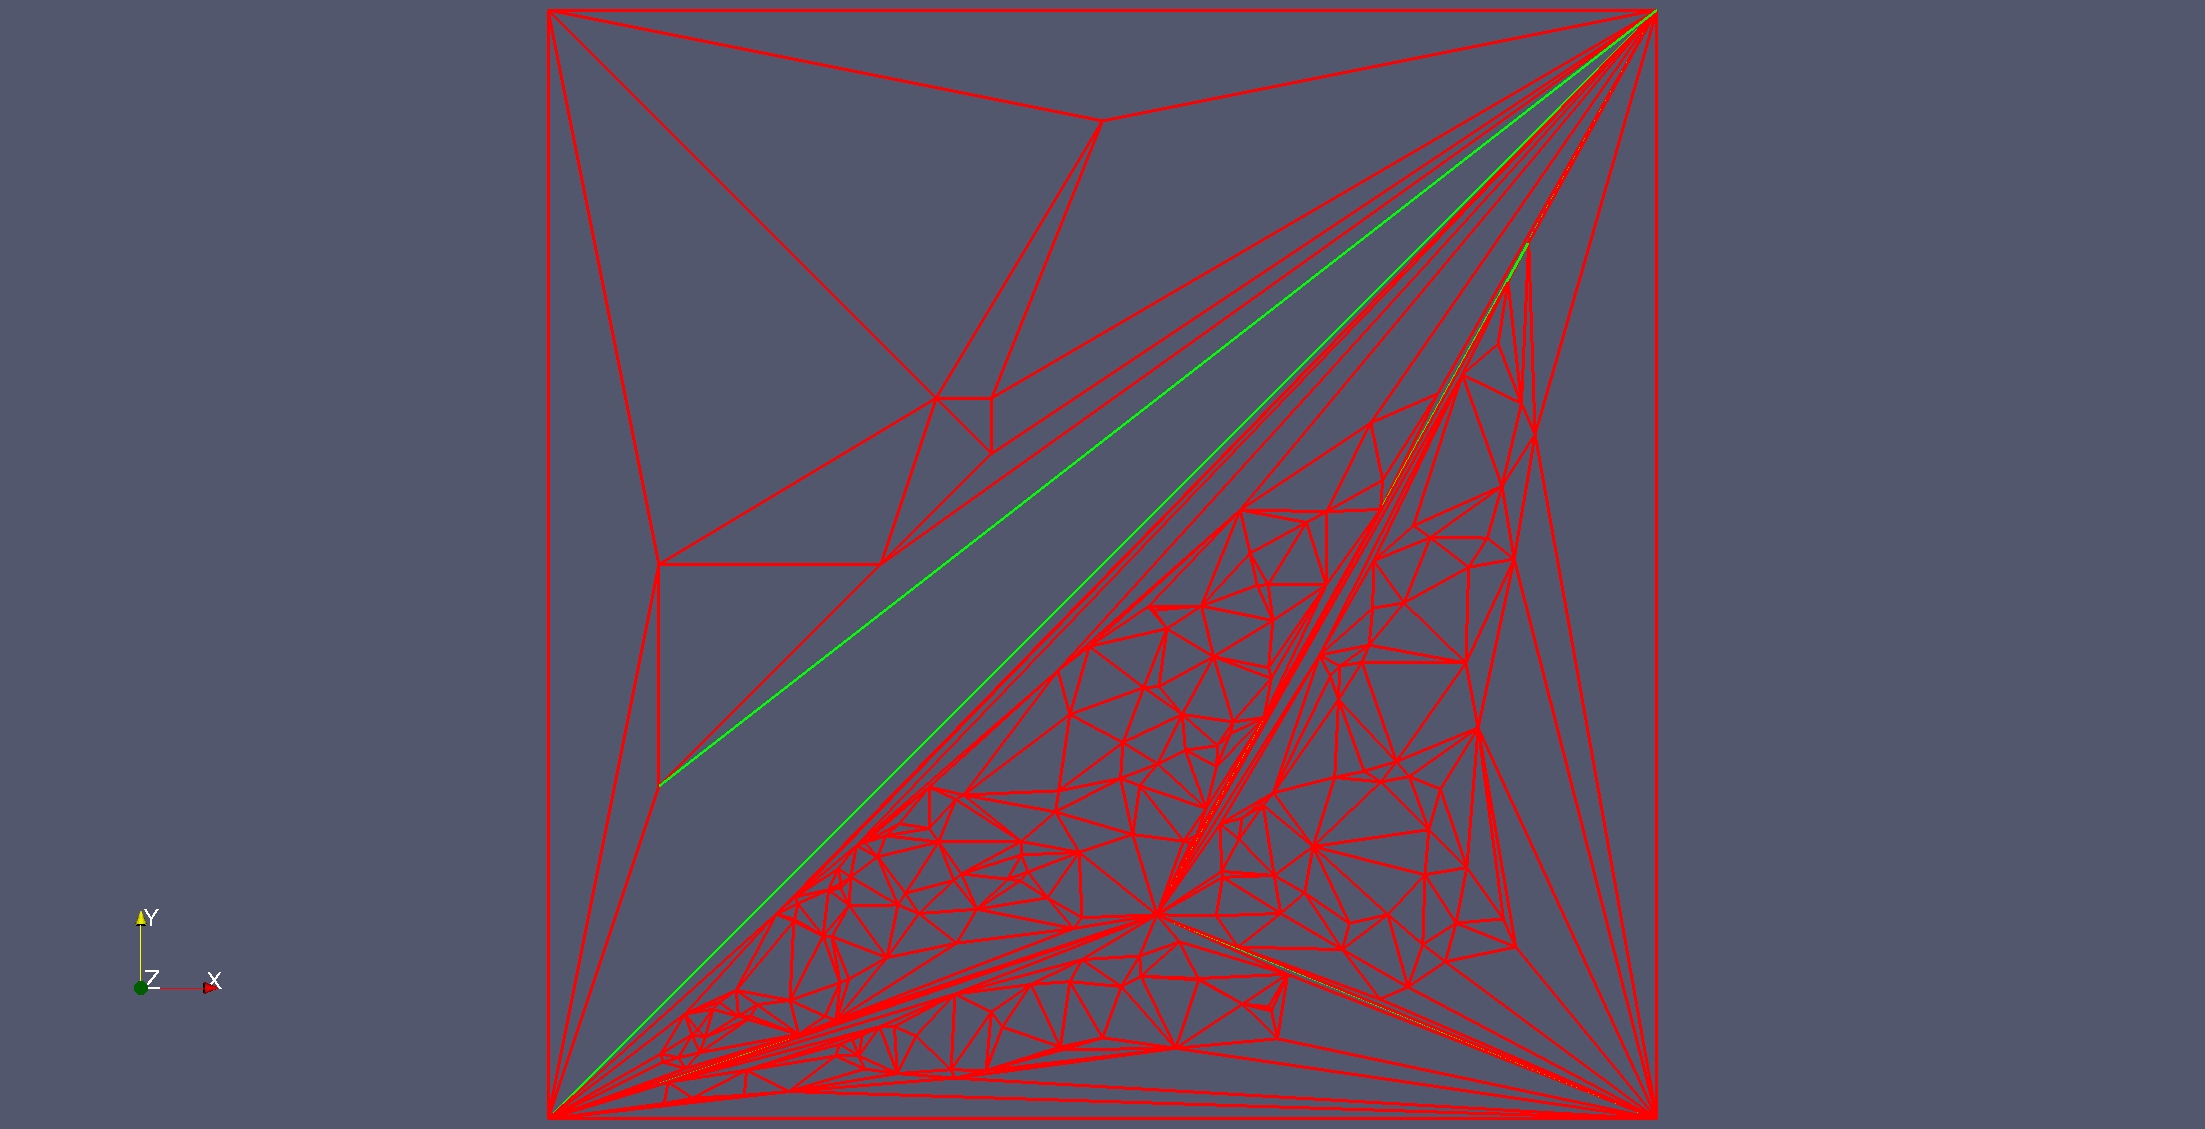
\includegraphics[scale=0.35, viewport=500 0 1680 1129, clip]{segments.jpg}
\caption{Maillage Delaunay contraint contenant cinq segments (coloriés en vert, sous Paraview), obtenu par modification de la triangulation de la figure \ref{two_segments}. On remarque la présence de triangles très plats près de ceux-ci, à tel point que les trois nouveaux segments sont chacun presque confondus avec d'autres arêtes.}\label{five_segments}
\end{center}
\end{figure}




\begin{figure}[htbp]
\begin{center}
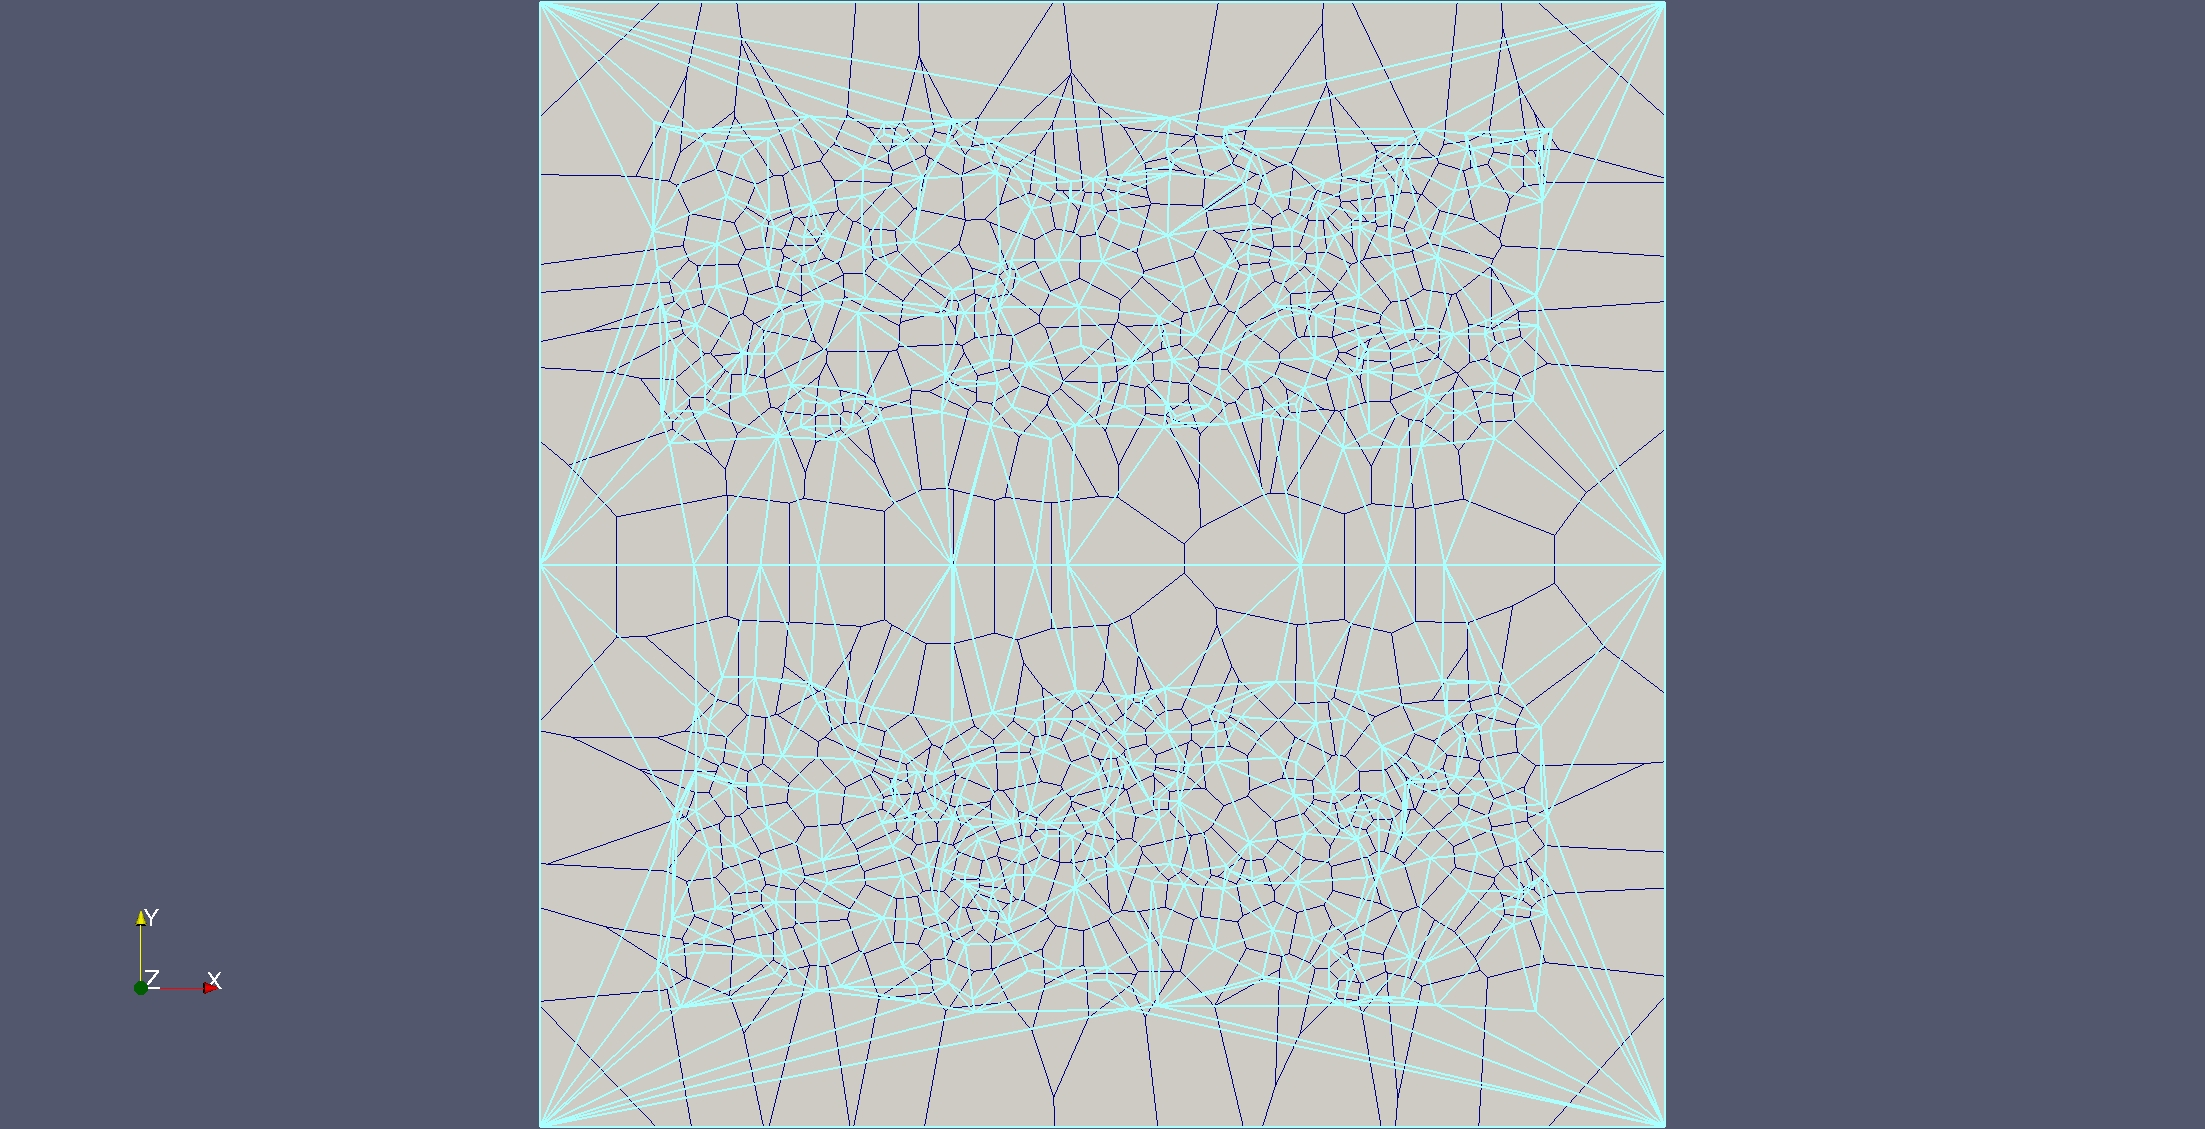
\includegraphics[scale=0.35, viewport=530 0 1680 1129, clip]{del_vor.jpg}
\caption{Triangulation de Delaunay d'un carré avec segments disposés à la médiane horizontale (arêtes en bleu clair) et diagramme de Voronoï correspondant (arêtes en bleu foncé) (image obtenue avec Paraview).}
\label{del_vor}
\end{center}
\end{figure}


\begin{center}
\begin{figure}[htbp]
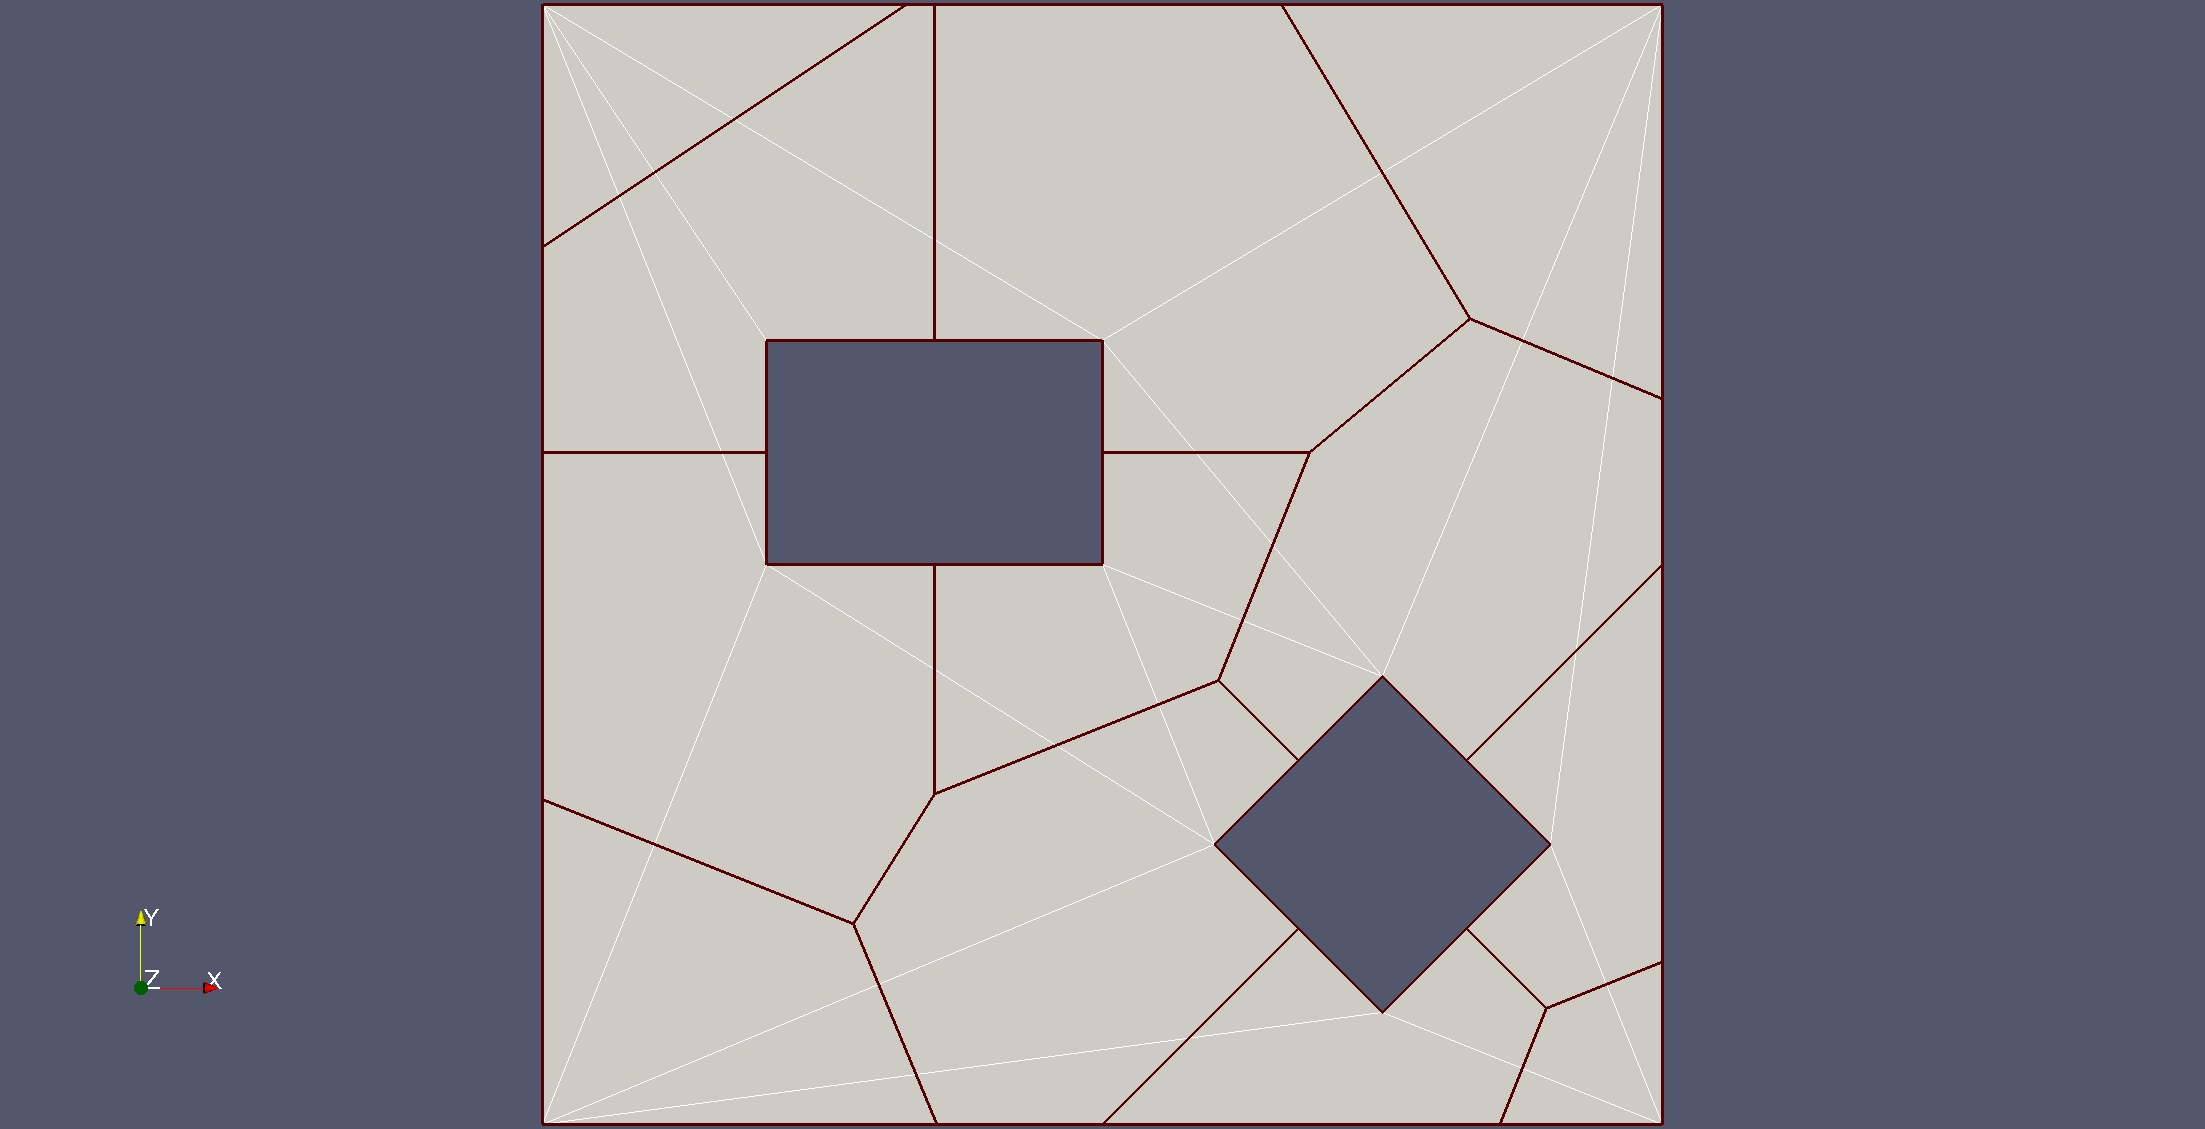
\includegraphics[scale=0.35, viewport=530 0 1680 1129, clip]{sq_del_vor.jpg}
\caption{Domaine non convexe (en gris) : triangulation de Delaunay (arêtes en blanc) et diagramme de Voronoï étendu correspondant (arêtes en marron) (image obtenue avec Paraview). Les cellules de Voronoï ne sont pas nécessairement convexes.}
\label{sq_del_vor}
\end{figure}
\end{center}
\clearpage

\section{Références}
\vspace*{1cm}

\bibliographystyle{plain}
\begin{btSect}{doc}
\section*{Bibliographie}
\btPrintCited
\end{btSect}
\label{biblio}

\bibliographystyle{plain}
\begin{btSect}{software}
\section*{Logiciels}
\btPrintCited
\end{btSect}
\label{software}

\bibliographystyle{plain}
\begin{btSect}{additional}
\section*{Seconde bibliographie}
%\btPrintCited
\btPrintNotCited
\end{btSect}
\label{second_biblio}


\end{document}
